% Chapter 8: Modern Extensions
% Harvard-quality academic presentation
% Bachelor program, Bucharest University of Economic Studies

\documentclass[9pt, aspectratio=169, t]{beamer}

% Ensure content fits on slides
\setbeamersize{text margin left=8mm, text margin right=8mm}

%=============================================================================
% THEME AND STYLE CONFIGURATION
%=============================================================================
\usetheme{default}
% Using default theme for clean header/footer control

% Color Palette (matching Redispatch PDF)
\definecolor{MainBlue}{RGB}{26, 58, 110}
\definecolor{AccentBlue}{RGB}{26, 58, 110}
\definecolor{IDAred}{RGB}{205, 0, 0}
\definecolor{DarkGray}{RGB}{51, 51, 51}
\definecolor{MediumGray}{RGB}{128, 128, 128}
\definecolor{LightGray}{RGB}{248, 248, 248}
\definecolor{VeryLightGray}{RGB}{235, 235, 235}
\definecolor{KeynoteGray}{RGB}{218, 218, 218}
\definecolor{SectionGray}{RGB}{120, 120, 120}
\definecolor{FooterGray}{RGB}{100, 100, 100}
\definecolor{Crimson}{RGB}{220, 53, 69}
\definecolor{Forest}{RGB}{46, 125, 50}
\definecolor{Amber}{RGB}{181, 133, 63}
\definecolor{Orange}{RGB}{230, 126, 34}
\definecolor{Purple}{RGB}{142, 68, 173}

% Gradient background (exact Keynote 315° gradient: white to RGB 218,218,218)
\setbeamertemplate{background}{%
    \begin{tikzpicture}[remember picture, overlay]
        \shade[shading=axis, shading angle=315,
        top color=white, bottom color=KeynoteGray]
        (current page.south west) rectangle (current page.north east);
    \end{tikzpicture}%
}
% Fallback solid color for compatibility
\setbeamercolor{background canvas}{bg=}

\setbeamercolor{palette primary}{bg=MainBlue, fg=white}
\setbeamercolor{palette secondary}{bg=MainBlue!85, fg=white}
\setbeamercolor{palette tertiary}{bg=MainBlue!70, fg=white}
\setbeamercolor{structure}{fg=MainBlue}
\setbeamercolor{title}{fg=IDAred}
\setbeamercolor{frametitle}{fg=IDAred, bg=}
\setbeamercolor{block title}{bg=MainBlue, fg=white}
\setbeamercolor{block body}{bg=VeryLightGray, fg=DarkGray}
\setbeamercolor{block title alerted}{bg=Crimson, fg=white}
\setbeamercolor{block body alerted}{bg=Crimson!8, fg=DarkGray}
\setbeamercolor{block title example}{bg=Forest, fg=white}
\setbeamercolor{block body example}{bg=Forest!8, fg=DarkGray}
\setbeamercolor{item}{fg=MainBlue}

% Footer colors (override Madrid theme blue)
\setbeamercolor{author in head/foot}{fg=FooterGray, bg=}
\setbeamercolor{title in head/foot}{fg=FooterGray, bg=}
\setbeamercolor{date in head/foot}{fg=FooterGray, bg=}
\setbeamercolor{section in head/foot}{fg=FooterGray, bg=}
\setbeamercolor{subsection in head/foot}{fg=FooterGray, bg=}

% Bullet styles (apply everywhere including blocks)
\setbeamertemplate{itemize item}{\color{MainBlue}$\boxdot$}
\setbeamertemplate{itemize subitem}{\color{MainBlue}$\blacktriangleright$}
\setbeamertemplate{itemize subsubitem}{\color{MainBlue}\tiny$\bullet$}
\setbeamertemplate{itemize/enumerate body begin}{\normalsize}
\setbeamertemplate{itemize/enumerate subbody begin}{\normalsize}

% Item spacing - compact style
\setlength{\leftmargini}{10pt}       % Level 1: minimal indent
\setlength{\leftmarginii}{10pt}      % Level 2: minimal additional indent
% Compact list spacing (zero extra space before/after lists in blocks)
\makeatletter
\def\@listi{\leftmargin\leftmargini \topsep 0pt \parsep 0pt \itemsep 0pt}
\def\@listii{\leftmargin\leftmarginii \topsep 0pt \parsep 0pt \itemsep 0pt}
\makeatother

\setbeamertemplate{navigation symbols}{}

%=============================================================================
% CUSTOM HEADLINE
%=============================================================================
\setbeamertemplate{headline}{%
    \vskip10pt%
    \hbox to \paperwidth{%
        \hskip0.5cm%
        {\small\color{FooterGray}\renewcommand{\hyperlink}[2]{##2}\insertsectionhead}%
        \hfill%
        \textcolor{FooterGray}{\small\insertframenumber}%
        \hskip0.5cm%
    }%
    \vskip4pt%
    {\color{FooterGray}\hrule height 0.4pt}%
}

%=============================================================================
% CUSTOM FOOTER
%=============================================================================
\usepackage{fontawesome5}

\setbeamertemplate{footline}{%
    {\color{FooterGray}\hrule height 0.4pt}%
    \vskip4pt%
    \hbox to \paperwidth{%
        \hskip0.5cm%
        \textcolor{FooterGray}{\small Time Series Analysis and Forecasting}%
        \hfill%
        \raisebox{-0.1em}{%
            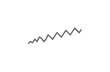
\begin{tikzpicture}[x=0.08em, y=0.08em, line width=0.4pt]
                \draw[FooterGray] (0,3) -- (1,4) -- (2,3.5) -- (3,5) -- (4,4) -- (5,6) -- (6,5.5) -- (7,4) -- (8,5) -- (9,7) -- (10,6) -- (11,5) -- (12,6.5) -- (13,8) -- (14,7) -- (15,6) -- (16,7.5) -- (17,9) -- (18,8) -- (19,7) -- (20,8.5) -- (21,10) -- (22,9) -- (23,8) -- (24,9.5);
            \end{tikzpicture}%
        }%
        \hskip0.5cm%
    }%
    \vskip6pt%
}

%=============================================================================
% PACKAGES
%=============================================================================
\usepackage[utf8]{inputenc}
\usepackage[T1]{fontenc}
\usepackage{amsmath, amssymb, amsthm}
\usepackage{mathtools}
\usepackage{bm}
\usepackage{tikz}
\usetikzlibrary{arrows.meta, positioning, shapes, calc, decorations.pathreplacing, shadings}
\usepackage{booktabs}
\usepackage{multirow}
\usepackage{array}
\usepackage{graphicx}
\usepackage{hyperref}
\usepackage{colortbl}
\hypersetup{colorlinks=true, linkcolor=MainBlue, urlcolor=MainBlue}
\graphicspath{{../../logos/}{../../charts/}{../../photos/}}
\hfuzz=2pt  % Suppress tiny overfull warnings (<2pt)
\vfuzz=2pt  % Suppress tiny vertical overfull warnings (<2pt)

%=============================================================================
% QUANTLET COMMAND
%=============================================================================
\newcommand{\quantlet}[2]{%
    \hfill\href{#2}{%
        \raisebox{-0.15em}{\includegraphics[height=0.7em]{ql_logo.png}}%
        \textcolor{MainBlue}{\tiny\ #1}%
    }%
}

%=============================================================================
% CUSTOM TITLE PAGE
%=============================================================================
\defbeamertemplate*{title page}{hybrid}[1][]
{
    \vspace{0.2cm}
    % Logos row - top header (with clickable links)
    \begin{center}
        \href{https://www.ase.ro}{\includegraphics[height=1.0cm]{ase_logo.png}}\hspace{0.3cm}%
        \href{https://theida.net}{\includegraphics[height=1.0cm]{ida_logo.png}}\hspace{0.3cm}%
        \href{https://blockchain-research-center.com}{\includegraphics[height=1.0cm]{brc_logo.png}}\hspace{0.3cm}%
        \href{https://www.ai4efin.ase.ro}{\includegraphics[height=1.0cm]{ai4efin_logo.png}}\hspace{0.3cm}%
        \href{https://ipe.ro/new}{\includegraphics[height=1.0cm]{acad_logo.png}}\hspace{0.3cm}%
        \href{https://www.digital-finance-msca.com}{\includegraphics[height=1.0cm]{msca_logo.png}}%
    \end{center}

    \vspace{0.6cm}

    % Main title with Q logos on sides (with clickable links)
    \begin{center}
        \begin{minipage}{0.1\textwidth}
            \centering
            \href{https://quantlet.com}{\includegraphics[height=1.1cm]{ql_logo.png}}
        \end{minipage}%
        \begin{minipage}{0.78\textwidth}
            \centering
            {\LARGE\bfseries\usebeamercolor[fg]{title}\inserttitle}

            \vspace{0.3cm}

            {\usebeamerfont{subtitle}\usebeamercolor[fg]{title}\insertsubtitle}
        \end{minipage}%
        \begin{minipage}{0.1\textwidth}
            \centering
            \href{https://quantinar.com}{\includegraphics[height=1.1cm]{qr_logo.png}}
        \end{minipage}
    \end{center}

    \vspace{0.6cm}

    % Authors (left aligned)
    \hspace{0.5cm}{\usebeamerfont{author}\insertauthor}

    \vspace{0.3cm}

    % Institute/Affiliations (left aligned)
    \hspace{0.5cm}\begin{minipage}[t]{0.9\textwidth}
        \raggedright\small\insertinstitute
    \end{minipage}
}

%=============================================================================
% THEOREM ENVIRONMENTS
%=============================================================================
\theoremstyle{definition}
\setbeamertemplate{theorems}[numbered]
\newtheorem{defn}{Definition}
\newtheorem{thm}{Theorem}
\newtheorem{prop}{Proposition}
\newtheorem{rmk}{Remark}

%=============================================================================
% CUSTOM COMMANDS
%=============================================================================
\newcommand{\E}{\mathbb{E}}
\newcommand{\Var}{\text{Var}}
\newcommand{\Cov}{\text{Cov}}
\newcommand{\Corr}{\text{Corr}}
\newcommand{\R}{\mathbb{R}}
\newcommand{\N}{\mathbb{N}}
\newcommand{\Z}{\mathbb{Z}}
\newcommand{\B}{\mathbf{B}}
\newcommand{\imark}{\textcolor{MainBlue}{\textbullet}}
\newcommand{\RMSE}{\text{RMSE}}
\newcommand{\MAE}{\text{MAE}}
\newcommand{\MAPE}{\text{MAPE}}

%=============================================================================
% TITLE INFORMATION
%=============================================================================
\title[Time Series Analysis]{Time Series Analysis and Forecasting}
\subtitle{Chapter 8: Modern Extensions}
\author[D.T. Pele]{Daniel Traian PELE}
\institute{Bucharest University of Economic Studies\\
IDA Institute Digital Assets\\
Blockchain Research Center\\
AI4EFin Artificial Intelligence for Energy Finance\\
Romanian Academy, Institute for Economic Forecasting\\
MSCA Digital Finance}
\date{}

%=============================================================================
% CENTRED MINIPAGE
%=============================================================================
\newenvironment{cminipage}[1]{%
    \par\noindent\hfill\begin{minipage}{#1}\ignorespaces
}{%
    \end{minipage}\hfill\null\par
}

\begin{document}

% Title page (no header/footer)
{
\setbeamertemplate{headline}{}
\setbeamertemplate{footline}{}
\begin{frame}
    \titlepage
\end{frame}
}

%=============================================================================
% LEARNING OBJECTIVES
%=============================================================================
\begin{frame}{Learning Objectives}
    \begin{cminipage}{0.95\textwidth}
    \begin{block}{By the end of this chapter, you will be able to:}
        \begin{itemize}\setlength{\itemsep}{2pt}
            \item[\textcolor{MainBlue}{\textbf{1.}}] \textbf{Understand} long memory and fractional integration
            \item[\textcolor{MainBlue}{\textbf{2.}}] \textbf{Distinguish} between short and long memory processes
            \item[\textcolor{MainBlue}{\textbf{3.}}] \textbf{Estimate} the fractional parameter $d$ using GPH, Local Whittle, and MLE
            \item[\textcolor{MainBlue}{\textbf{4.}}] \textbf{Apply} Random Forest for time series forecasting
            \item[\textcolor{MainBlue}{\textbf{5.}}] \textbf{Build} LSTM networks for sequential data
            \item[\textcolor{MainBlue}{\textbf{6.}}] \textbf{Compare} classical vs ML model performance
            \item[\textcolor{MainBlue}{\textbf{7.}}] \textbf{Choose} the appropriate method based on data characteristics
            \item[\textcolor{MainBlue}{\textbf{8.}}] \textbf{Implement} ARFIMA, Random Forest, and LSTM in Python
        \end{itemize}
    \end{block}
    \end{cminipage}
\end{frame}

%=============================================================================
% TABLE OF CONTENTS
%=============================================================================
\begin{frame}{Outline}
    \setbeamertemplate{section in toc}{\color{MainBlue}$\boxdot$~\inserttocsection}
    \tableofcontents
\end{frame}

%=============================================================================
\section{Motivation}
%=============================================================================

\begin{frame}{From Classical Models to Machine Learning}
    \begin{cminipage}{0.95\textwidth}
    \begin{block}{The Evolution of Time Series Methods}
        \begin{itemize}\setlength{\itemsep}{0pt}
            \item \textbf{Classical ARIMA} (Box \& Jenkins, 1970) --- revolutionized forecasting but has limitations:
            \begin{itemize}\setlength{\itemsep}{0pt}
                \item Assumes \textbf{short memory}: autocorrelations decay exponentially
                \item \textbf{Linear} relationships only --- cannot capture complex dynamics
                \item Requires \textbf{stationarity} through integer differencing
            \end{itemize}
        \end{itemize}
    \end{block}

    \vspace{0.1cm}

    \begin{alertblock}{Three Paradigm Shifts}
        \begin{itemize}\setlength{\itemsep}{0pt}
            \item \textbf{ARFIMA} (Granger \& Joyeux, 1980)
            \begin{itemize}\setlength{\itemsep}{0pt}
                \item Fractional integration for long memory processes
            \end{itemize}
            \item \textbf{Random Forest} (Breiman, 2001)
            \begin{itemize}\setlength{\itemsep}{0pt}
                \item Ensemble learning for nonlinear relationships
            \end{itemize}
            \item \textbf{LSTM} (Hochreiter \& Schmidhuber, 1997)
            \begin{itemize}\setlength{\itemsep}{0pt}
                \item Deep learning for complex sequential patterns
            \end{itemize}
        \end{itemize}
    \end{alertblock}
    \end{cminipage}
\end{frame}

\begin{frame}{When to Use Each Method?}
    \begin{cminipage}{0.95\textwidth}
    \vspace{-0.2cm}
    \begin{center}
    {\small
    \begin{tabular}{l|c|c|c|c}
        \toprule
        \textbf{Feature} & \textbf{ARIMA} & \textbf{ARFIMA} & \textbf{RF} & \textbf{LSTM} \\
        \midrule
        Long memory & $\times$ & $\checkmark$ & $\checkmark$ & $\checkmark$ \\
        Nonlinear relationships & $\times$ & $\times$ & $\checkmark$ & $\checkmark$ \\
        Interpretability & $\checkmark$ & $\checkmark$ & $\sim$ & $\times$ \\
        Small data & $\checkmark$ & $\checkmark$ & $\times$ & $\times$ \\
        Exogenous variables & $\checkmark$ & $\checkmark$ & $\checkmark$ & $\checkmark$ \\
        Uncertainty quantification & $\checkmark$ & $\checkmark$ & $\sim$ & $\times$ \\
        \bottomrule
    \end{tabular}
    }
    \end{center}

    \vspace{0.1cm}

    \begin{exampleblock}{Principle of Parsimony (Occam's Razor)}
        Start \textbf{simple} (ARIMA), then increase complexity only if justified by \textbf{out-of-sample} performance gains.
        {\footnotesize Makridakis et al.\ (2018) M4 Competition: simple methods often outperform complex ML models.}
    \end{exampleblock}
    \end{cminipage}
\end{frame}

%=============================================================================
\section{ARFIMA: Long Memory Models}
%=============================================================================

\begin{frame}{ACF Comparison: Short Memory vs Long Memory}
    \vspace{-0.2cm}
    {\footnotesize
    \begin{block}{Interpretation}
            \begin{itemize}\setlength{\itemsep}{0pt}
                \item \textbf{Data}: Simulated AR(1) with $\phi=0.8$ and ARFIMA(0,$d$,0) with $d=0.35$ ($n=1000$)
                \item \textbf{Left}: AR(1) --- autocorrelations decay exponentially (short memory)
                \item \textbf{Right}: ARFIMA with $d=0.35$ --- autocorrelations decay hyperbolically (long memory)
            \end{itemize}
        \end{block}
    }
    \begin{center}
        \includegraphics[width=0.95\textwidth, height=0.50\textheight, keepaspectratio]{ch8_acf_comparison.pdf}
    \end{center}
    \quantlet{TSA\_ch8\_acf\_comparison}{https://github.com/QuantLet/TSA/tree/main/TSA_ch8/TSA_ch8_acf_comparison}
\end{frame}

\begin{frame}{What is Long Memory?}
    \begin{cminipage}{0.95\textwidth}
    \vspace{-0.2cm}
    \begin{block}{Short Memory (ARMA)}
        \begin{itemize}\setlength{\itemsep}{0pt}
            \item \textbf{ACF Behavior}:
            \begin{itemize}\setlength{\itemsep}{0pt}
                \item Autocorrelations $\rho_k$ decay \textbf{exponentially}: $|\rho_k| \leq C \cdot r^k$, $r < 1$
                \item Finite sum: $\sum_{k=0}^{\infty} |\rho_k| < \infty$
            \end{itemize}
            \item \textbf{Implication}: Shock effects disappear quickly
        \end{itemize}
    \end{block}
    \begin{alertblock}{Long Memory (ARFIMA)}
        \begin{itemize}\setlength{\itemsep}{0pt}
            \item \textbf{ACF Behavior}:
            \begin{itemize}\setlength{\itemsep}{0pt}
                \item Autocorrelations decay \textbf{hyperbolically}: $\rho_k \sim C \cdot k^{2d-1}$
                \item Infinite sum: $\sum_{k=0}^{\infty} |\rho_k| = \infty$
            \end{itemize}
            \item \textbf{Implication}: Shock effects persist for a long time
        \end{itemize}
    \end{alertblock}
    \begin{exampleblock}{Examples}
        Financial volatility, river flows, network traffic, inflation, climate data
    \end{exampleblock}
    \end{cminipage}
\end{frame}

\begin{frame}{The ARFIMA(p,d,q) Model}
    \begin{cminipage}{0.95\textwidth}
    \vspace{-0.3cm}
    {\small
    \begin{defn}[ARFIMA --- Granger \& Joyeux (1980), Hosking (1981)]
        A process $\{Y_t\}$ follows an \textbf{ARFIMA(p,d,q)} model if:
        $\phi(L)(1-L)^d Y_t = \theta(L)\varepsilon_t$
        where $d \in (-0.5, 0.5)$ is the \textbf{fractional differencing parameter}.
    \end{defn}

    \vspace{0.1cm}

    \begin{block}{Fractional Differencing Operator}
        $(1-L)^d = \sum_{k=0}^{\infty} \binom{d}{k}(-L)^k = 1 - dL - \frac{d(1-d)}{2!}L^2 - \frac{d(1-d)(2-d)}{3!}L^3 - \cdots$
    \end{block}

    \vspace{0.1cm}

    {\small
    \begin{itemize}\setlength{\itemsep}{0pt}
        \item $d = 0$: Standard ARMA (short memory)
        \item $0 < d < 0.5$: Long memory, stationary
        \item $d = 0.5$: Stationarity boundary
        \item $0.5 \leq d < 1$: Non-stationary, mean-reverting
        \item $d = 1$: Random walk (standard ARIMA)
    \end{itemize}
    }
    }
    \end{cminipage}
\end{frame}

\begin{frame}{Effect of Parameter $d$ on ACF}
    \vspace{-0.2cm}
    {\footnotesize
    \begin{block}{Interpretation}
            \begin{itemize}\setlength{\itemsep}{0pt}
                \item \textbf{Data}: Simulated ARFIMA(0,$d$,0) for $d \in \{0.1, 0.2, 0.3, 0.4\}$ ($n=1000$)
                \item The higher $d$, the slower autocorrelations decay
                \item As $d \to 0.5$, autocorrelations remain significant even at very large lags
            \end{itemize}
        \end{block}
    }
    \begin{center}
        \includegraphics[width=0.95\textwidth, height=0.50\textheight, keepaspectratio]{ch8_arfima_d_effect.pdf}
    \end{center}
    \quantlet{TSA\_ch8\_arfima\_d\_effect}{https://github.com/QuantLet/TSA/tree/main/TSA_ch8/TSA_ch8_arfima_d_effect}
\end{frame}

\begin{frame}{Interpreting the Parameter $d$}
    \begin{cminipage}{0.95\textwidth}
    \begin{center}
    \begin{tabular}{c|l|l}
        \toprule
        \textbf{Value of $d$} & \textbf{ACF Behavior} & \textbf{Interpretation} \\
        \midrule
        $d = 0$ & Exponential decay & Short memory \\
        $0 < d < 0.5$ & Hyperbolic decay & Long memory, stationary \\
        $d = 0.5$ & Non-summable ACF & At the boundary \\
        $0.5 < d < 1$ & Very slow decay & Long memory, non-stationary \\
        $d = 1$ & ACF = 1 (constant) & Random walk \\
        \bottomrule
    \end{tabular}
    \end{center}

    \vspace{0.3cm}

    \begin{block}{Hurst Parameter $H$}
        Relationship with Hurst exponent: $d = H - 0.5$
        \begin{itemize}\setlength{\itemsep}{0pt}
            \item $H = 0.5$: Random walk (no memory)
            \item $H > 0.5$: Persistence (trend-following)
            \item $H < 0.5$: Anti-persistence (mean-reverting)
        \end{itemize}
    \end{block}
    \end{cminipage}
\end{frame}

\begin{frame}{Hurst Exponent: Visual Interpretation}
    \vspace{-0.2cm}
    {\scriptsize
    \begin{block}{Interpretation}
        \begin{itemize}\setlength{\itemsep}{0pt}
            \item \textbf{Data}: Simulated fractional Brownian motion with $H \in \{0.3, 0.5, 0.7\}$
            \item \textbf{H $<$ 0.5}: Mean-reverting \quad \textbf{H = 0.5}: Random walk \quad \textbf{H $>$ 0.5}: Persistent
        \end{itemize}
    \end{block}
    }
    \begin{center}
        \includegraphics[width=0.95\textwidth, height=0.50\textheight, keepaspectratio]{ch8_hurst_interpretation.pdf}
    \end{center}
    \quantlet{TSA\_ch8\_hurst\_interpretation}{https://github.com/QuantLet/TSA/tree/main/TSA_ch8/TSA_ch8_hurst_interpretation}
\end{frame}

\begin{frame}{ARIMA vs ARFIMA: Memory Decay Patterns}
    \vspace{-0.2cm}
    {\footnotesize
    \begin{block}{Interpretation}
            \begin{itemize}\setlength{\itemsep}{0pt}
                \item \textbf{Data}: Simulated ARIMA(1,1,1) vs ARFIMA(1,$d$,1) with $d=0.35$
                \item \textbf{ARIMA} (left): ACF decays \textbf{exponentially} -- shocks are quickly ``forgotten''
                \item \textbf{ARFIMA} (right, $d=0.35$): ACF decays \textbf{hyperbolically} -- shocks persist for long periods
            \end{itemize}
        \end{block}
    }
    \begin{center}
        \includegraphics[width=0.95\textwidth, height=0.50\textheight, keepaspectratio]{ch8_arima_vs_arfima.pdf}
    \end{center}
    \quantlet{TSA\_ch8\_arima\_vs\_arfima}{https://github.com/QuantLet/TSA/tree/main/TSA_ch8/TSA_ch8_arima_vs_arfima}
\end{frame}

\begin{frame}{EUR/RON Long Memory Analysis}
    \vspace{-0.2cm}
    {\footnotesize
    \begin{block}{Interpretation}
            \begin{itemize}\setlength{\itemsep}{0pt}
                \item \textbf{Data}: EUR/RON daily exchange rate (Yahoo Finance, 2015--2025)
                \item \textbf{Returns}: $H \approx 0.50$, $d \approx 0$ -- short memory
                \item \textbf{Squared returns}: $H \approx 0.65$, $d \approx 0.15$ -- long memory in volatility
            \end{itemize}
        \end{block}
    }
    \begin{center}
        \includegraphics[width=0.95\textwidth, height=0.50\textheight, keepaspectratio]{ch8_eurron_long_memory.pdf}
    \end{center}
    \quantlet{TSA\_ch8\_eurron\_long\_memory}{https://github.com/QuantLet/TSA/tree/main/TSA_ch8/TSA_ch8_eurron_long_memory}
\end{frame}

\begin{frame}{ARFIMA Example: S\&P 500 Realized Volatility}
    \vspace{-0.2cm}
    {\footnotesize
    \begin{block}{Estimation Results}
            \begin{itemize}\setlength{\itemsep}{0pt}
                \item \textbf{Data}: S\&P 500 daily returns (Yahoo Finance, 2015--2024)
                \item Hurst: $H = 0.92$, $d = H - 0.5 = 0.42$ -- strong long memory in realized volatility
            \end{itemize}
        \end{block}
        \begin{alertblock}{Key Insight}
            Volatility has \textbf{long memory} -- shocks persist longer than ARMA; use ARFIMA or FIGARCH!
        \end{alertblock}
    }
    \begin{center}
        \includegraphics[width=0.95\textwidth, height=0.42\textheight, keepaspectratio]{ch8_arfima_real_data.pdf}
    \end{center}
    \quantlet{TSA\_ch8\_arfima\_sp500}{https://github.com/QuantLet/TSA/tree/main/TSA_ch8/TSA_ch8_arfima_sp500}
\end{frame}

\begin{frame}{Real Example: Long Memory in Volatility}
    \vspace{-0.2cm}
    {\footnotesize
        \begin{block}{Interpretation}
            \begin{itemize}\setlength{\itemsep}{0pt}
                \item \textbf{Data}: S\&P 500 daily returns (Yahoo Finance, 2010--2025)
                \item \textbf{Stylized Fact}: Financial returns have short memory, but volatility ($|r_t|$) has long memory
                \item This is the basis for FIGARCH models
            \end{itemize}
        \end{block}
        }
    \begin{center}
        \includegraphics[width=0.95\textwidth, height=0.50\textheight, keepaspectratio]{ch8_volatility_long_memory.pdf}
    \end{center}
    \quantlet{TSA\_ch8\_volatility\_long\_memory}{https://github.com/QuantLet/TSA/tree/main/TSA_ch8/TSA_ch8_volatility_long_memory}
\end{frame}

\begin{frame}{Estimating the Parameter $d$}
    \vspace{-0.2cm}
    {\footnotesize
    \begin{block}{Estimation Methods}
        \begin{itemize}\setlength{\itemsep}{0pt}
            \item \textbf{GPH (Geweke-Porter-Hudak)}: Frequency-domain regression
            \begin{itemize}\setlength{\itemsep}{0pt}
                \item $\ln I(\omega_j) = c - d \cdot \ln\bigl(4\sin^2\frac{\omega_j}{2}\bigr) + \varepsilon_j$
            \end{itemize}
            \item \textbf{R/S (Rescaled Range)}: Hurst's method
            \begin{itemize}\setlength{\itemsep}{0pt}
                \item $\frac{R}{S}(n) \sim c \cdot n^H$
            \end{itemize}
            \item \textbf{MLE (Maximum Likelihood)}: Full ARFIMA estimation
            \item \textbf{Whittle}: Efficient frequency-domain approximation
        \end{itemize}
    \end{block}

    \vspace{0.2cm}

    {\footnotesize
    \begin{exampleblock}{Implementation}
        \begin{itemize}\setlength{\itemsep}{0pt}
            \item In Python: \texttt{arch} package, \texttt{statsmodels.tsa.arima.model.ARIMA} with \texttt{order=(p,d,q)} where $d$ can be fractional
        \end{itemize}
    \end{exampleblock}
    }
    }
\end{frame}


%=============================================================================
\section{Random Forest for Time Series}
%=============================================================================

\begin{frame}{Random Forest: Basic Concepts}
    \begin{cminipage}{0.95\textwidth}
    \begin{block}{What is Random Forest? (Breiman, 2001)}
        \begin{itemize}\setlength{\itemsep}{0pt}
            \item \textbf{Ensemble} of decision trees
            \item Each tree trained on a \textbf{bootstrap subset} of the data
            \item At each node, a \textbf{random} subset of features is selected
            \item Final prediction = \textbf{average} of all tree predictions
        \end{itemize}
    \end{block}

    \vspace{0.2cm}

    \begin{exampleblock}{Advantages for Time Series}
        \begin{itemize}\setlength{\itemsep}{0pt}
            \item Captures \textbf{nonlinear relationships}
            \item \textbf{Robust} to outliers and noise
            \item Does not require \textbf{stationarity}
            \item Provides \textbf{feature importance} (interpretability)
            \item Works well with \textbf{many variables}
        \end{itemize}
    \end{exampleblock}
    \end{cminipage}
\end{frame}

\begin{frame}{Feature Engineering: Illustration}
    \vspace{-0.2cm}
    {\footnotesize
    \begin{block}{Interpretation}
            \begin{itemize}\setlength{\itemsep}{0pt}
                \item \textbf{Data}: Germany daily electricity consumption (OPSD, 2012--2017)
                \item We transform the time series into features: lags, rolling statistics
                \item The RF model learns relationships between these and future values
            \end{itemize}
        \end{block}
    }
    \begin{center}
        \includegraphics[width=0.95\textwidth, height=0.50\textheight, keepaspectratio]{ch8_feature_engineering.pdf}
    \end{center}
    \quantlet{TSA\_ch8\_feature\_engineering}{https://github.com/QuantLet/TSA/tree/main/TSA_ch8/TSA_ch8_feature_engineering}
\end{frame}

\begin{frame}{Data Preparation for Random Forest}
    \begin{cminipage}{0.95\textwidth}
    \begin{block}{Feature Engineering for Time Series}
        \begin{enumerate}\setlength{\itemsep}{0pt}
            \item \textbf{Lag features}: $Y_{t-1}, Y_{t-2}, \ldots, Y_{t-p}$
            \item \textbf{Rolling statistics}: moving average, standard deviation
            \item \textbf{Calendar features}: day of week, month, season
            \item \textbf{Trend features}: time, quadratic trend
            \item \textbf{Exogenous variables}: economic indicators, events
        \end{enumerate}
    \end{block}

    \vspace{0.2cm}

    \begin{alertblock}{Warning: Data Leakage!}
        \begin{itemize}\setlength{\itemsep}{0pt}
            \item Do not use future information in features
            \item Train/test split: \textbf{temporal}, not random!
            \item Rolling statistics: compute only on \textbf{past} data
        \end{itemize}
    \end{alertblock}
    \end{cminipage}
\end{frame}


\begin{frame}{Random Forest: Forecast Example}
    \vspace{-0.2cm}
    {\scriptsize
    \begin{block}{Interpretation}
        \begin{itemize}\setlength{\itemsep}{0pt}
            \item \textbf{Data}: Germany daily electricity consumption (OPSD, 2012--2017)
            \item RF trained on historical data (blue) produces forecasts (red dashed) that closely track actual values (green)
        \end{itemize}
    \end{block}
    }
    \begin{center}
        \includegraphics[width=0.95\textwidth, height=0.50\textheight, keepaspectratio]{ch8_rf_prediction.pdf}
    \end{center}
    \quantlet{TSA\_ch8\_rf\_prediction}{https://github.com/QuantLet/TSA/tree/main/TSA_ch8/TSA_ch8_rf_prediction}
\end{frame}

\begin{frame}{Feature Importance and Interpretation}
    \begin{cminipage}{0.95\textwidth}
    \begin{block}{Feature Importance}
        \begin{itemize}\setlength{\itemsep}{0pt}
            \item \textbf{Mean Decrease Impurity (MDI)}: Impurity reduction at each split
            \item \textbf{Permutation Importance}: How much performance drops when a feature is randomly permuted
        \end{itemize}
    \end{block}

    \vspace{0.2cm}

    \begin{exampleblock}{Typical Interpretation for Time Series}
        \begin{itemize}\setlength{\itemsep}{0pt}
            \item \texttt{lag\_1} very important $\Rightarrow$ Strong autocorrelation
            \item \texttt{rolling\_mean} important $\Rightarrow$ Local trend matters
            \item \texttt{month} important $\Rightarrow$ Seasonality present
        \end{itemize}
    \end{exampleblock}

    \vspace{0.2cm}

    {\footnotesize
    \begin{block}{Code}
        \begin{itemize}\setlength{\itemsep}{0pt}
            \item \texttt{rf.feature\_importances\_} or \texttt{permutation\_importance(rf, X\_test, y\_test)}
        \end{itemize}
    \end{block}
    }
    \end{cminipage}
\end{frame}

%=============================================================================
\section{LSTM: Deep Learning for Time Series}
%=============================================================================

\begin{frame}{Researcher Spotlight: Hochreiter \& Schmidhuber}
    \vspace{-0.3cm}
    \begin{columns}[T]
        \begin{column}{0.22\textwidth}
            \centering
            \includegraphics[width=0.95\textwidth, height=0.20\textheight, keepaspectratio]{photo_sepp_hochreiter.jpg}
            \\[0.05cm]
            {\tiny\textcolor{MediumGray}{Sepp Hochreiter (*1967)}}\\[0.02cm]
            \href{https://en.wikipedia.org/wiki/Sepp_Hochreiter}{\faWikipediaW\ \textcolor{MainBlue}{\tiny Wikipedia}}
        \end{column}
        \begin{column}{0.76\textwidth}
            \begin{block}{Biography}
                {\footnotesize \begin{itemize}\setlength{\itemsep}{0pt}
                    \item \textbf{Sepp Hochreiter}: Austrian computer scientist, Professor at Johannes Kepler University Linz and head of ELLIS Unit Linz
                    \item \textbf{J\"{u}rgen Schmidhuber}: German-Swiss computer scientist, Scientific Director of IDSIA
                    \item Together they solved the vanishing gradient problem
                \end{itemize}}
            \end{block}
        \end{column}
    \end{columns}
    \vspace{-0.1cm}
    \begin{columns}[T]
        \begin{column}{0.22\textwidth}
            \centering
            \includegraphics[width=0.95\textwidth, height=0.20\textheight, keepaspectratio]{photo_juergen_schmidhuber.jpg}
            \\[0.05cm]
            {\tiny\textcolor{MediumGray}{J\"{u}rgen Schmidhuber (*1963)}}\\[0.02cm]
            \href{https://en.wikipedia.org/wiki/J\%C3\%BCrgen_Schmidhuber}{\faWikipediaW\ \textcolor{MainBlue}{\tiny Wikipedia}}
        \end{column}
        \begin{column}{0.76\textwidth}
            \begin{exampleblock}{Key Contributions}
                {\footnotesize
                \begin{itemize}\setlength{\itemsep}{0pt}
                    \item \textbf{Long Short-Term Memory} (LSTM, 1997) --- gated recurrent architecture solving the vanishing gradient problem
                    \item \textbf{Vanishing gradient analysis} (Hochreiter, 1991) --- identified the fundamental training problem in deep networks
                    \item \textbf{Forget gate} extension (Gers et al., 2000) --- crucial addition enabling practical LSTM use
                    \item Foundation for modern sequence modeling in NLP, speech, and time series
                \end{itemize}}
            \end{exampleblock}
        \end{column}
    \end{columns}
\end{frame}

\begin{frame}{From Biological to Artificial Neurons}
    \vspace{-0.2cm}
    {\scriptsize
    \begin{block}{The Analogy}
        \begin{itemize}\setlength{\itemsep}{0pt}
            \item \textbf{Dendrites} $\rightarrow$ \textbf{Inputs} $x_i$ \quad \textbf{Synapses} $\rightarrow$ \textbf{Weights} $w_i$ \quad \textbf{Soma} $\rightarrow$ \textbf{Sum + Activation} \quad \textbf{Axon} $\rightarrow$ \textbf{Output} $y$
        \end{itemize}
    \end{block}
    }
    \begin{center}
        \includegraphics[width=0.95\textwidth, height=0.50\textheight, keepaspectratio]{ch8_neuron_comparison.pdf}
    \end{center}
    \quantlet{TSA\_ch8\_neuron\_comparison}{https://github.com/QuantLet/TSA/tree/main/TSA_ch8/TSA_ch8_neuron_comparison}
\end{frame}

\begin{frame}{Recurrent Neural Networks (RNN)}
    \begin{block}{Basic Idea}
        \begin{itemize}\setlength{\itemsep}{0pt}
            \item Networks that process \textbf{sequences} of data
            \item Have \textbf{internal memory} (hidden state)
            \item Current state depends on input + previous state
        \end{itemize}
    \end{block}

    \vspace{0.1cm}

    \begin{center}
    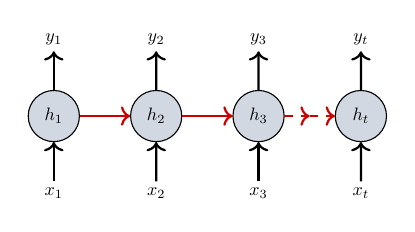
\begin{tikzpicture}[scale=0.65, transform shape]
        \node[draw, circle, minimum size=1cm, fill=MainBlue!20] (h1) at (0,0) {$h_1$};
        \node[draw, circle, minimum size=1cm, fill=MainBlue!20] (h2) at (2,0) {$h_2$};
        \node[draw, circle, minimum size=1cm, fill=MainBlue!20] (h3) at (4,0) {$h_3$};
        \node[draw, circle, minimum size=1cm, fill=MainBlue!20] (ht) at (6,0) {$h_t$};

        \node (x1) at (0,-1.5) {$x_1$};
        \node (x2) at (2,-1.5) {$x_2$};
        \node (x3) at (4,-1.5) {$x_3$};
        \node (xt) at (6,-1.5) {$x_t$};

        \node (y1) at (0,1.5) {$y_1$};
        \node (y2) at (2,1.5) {$y_2$};
        \node (y3) at (4,1.5) {$y_3$};
        \node (yt) at (6,1.5) {$y_t$};

        \draw[->, thick] (x1) -- (h1);
        \draw[->, thick] (x2) -- (h2);
        \draw[->, thick] (x3) -- (h3);
        \draw[->, thick] (xt) -- (ht);

        \draw[->, thick] (h1) -- (y1);
        \draw[->, thick] (h2) -- (y2);
        \draw[->, thick] (h3) -- (y3);
        \draw[->, thick] (ht) -- (yt);

        \draw[->, thick, IDAred] (h1) -- (h2);
        \draw[->, thick, IDAred] (h2) -- (h3);
        \draw[->, thick, IDAred, dashed] (h3) -- (5,0);
        \draw[->, thick, IDAred, dashed] (5,0) -- (ht);
    \end{tikzpicture}
    \end{center}

    \begin{alertblock}{Problem: Vanishing Gradient}
        \begin{itemize}\setlength{\itemsep}{0pt}
            \item Simple RNNs ``forget'' information from the distant past.
        \end{itemize}
    \end{alertblock}
\end{frame}

\begin{frame}{RNN Unfolded in Time}
    \begin{center}
        \includegraphics[width=0.95\textwidth, height=0.78\textheight, keepaspectratio]{ch8_rnn_unfolded.pdf}
    \end{center}
    \quantlet{TSA\_ch8\_rnn\_unfolded}{https://github.com/QuantLet/TSA/tree/main/TSA_ch8/TSA_ch8_rnn_unfolded}
\end{frame}

\begin{frame}{LSTM Cell: Detailed Diagram}

    \vspace{-0.2cm}
    \begin{center}
        \includegraphics[width=0.95\textwidth, height=0.73\textheight, keepaspectratio]{ch8_lstm_cell.pdf}
    \end{center}
    \vspace{-0.3cm}
    {\footnotesize
    \begin{columns}[T]
        \begin{column}{0.32\textwidth}
            \textbf{Forget Gate} $f_t$\\
            $\sigma(W_f[h_{t-1}, x_t] + b_f)$\\
            What to forget?
        \end{column}
        \begin{column}{0.32\textwidth}
            \textbf{Input Gate} $i_t$\\
            $\sigma(W_i[h_{t-1}, x_t] + b_i)$\\
            What to store?
        \end{column}
        \begin{column}{0.32\textwidth}
            \textbf{Output Gate} $o_t$\\
            $\sigma(W_o[h_{t-1}, x_t] + b_o)$\\
            What to transmit?
        \end{column}
    \end{columns}
    }

    \quantlet{TSA\_ch8\_lstm\_cell}{https://github.com/QuantLet/TSA/tree/main/TSA_ch8/TSA_ch8_lstm_cell}
\end{frame}

\begin{frame}{LSTM: Long Short-Term Memory}
    \begin{cminipage}{0.95\textwidth}
    \vspace{-0.2cm}
    {\small
    \begin{block}{The LSTM Solution}
        \begin{itemize}\setlength{\itemsep}{0pt}
            \item \textbf{Concept}: Special cells with 3 gates that control information flow
            \item \textbf{Forget Gate} ($f_t$): What to forget from previous memory
            \item \textbf{Input Gate} ($i_t$): What new information to add
            \item \textbf{Output Gate} ($o_t$): What to send to output
        \end{itemize}
    \end{block}

    \vspace{-0.05cm}

    \begin{block}{LSTM Equations}
        \begin{itemize}\setlength{\itemsep}{0pt}
        \item {\footnotesize
        \begin{align*}
            f_t &= \sigma(W_f \cdot [h_{t-1}, x_t] + b_f) & \text{(Forget)} \\
            i_t &= \sigma(W_i \cdot [h_{t-1}, x_t] + b_i) & \text{(Input)} \\
            \tilde{C}_t &= \tanh(W_C \cdot [h_{t-1}, x_t] + b_C) & \text{(Candidate)} \\
            C_t &= f_t \odot C_{t-1} + i_t \odot \tilde{C}_t & \text{(Cell state)} \\
            o_t &= \sigma(W_o \cdot [h_{t-1}, x_t] + b_o) & \text{(Output)} \\
            h_t &= o_t \odot \tanh(C_t) & \text{(Hidden state)}
        \end{align*}
        }
        \end{itemize}
    \end{block}
    }
    \end{cminipage}
\end{frame}

\begin{frame}{LSTM Cell Architecture}
    \vspace{-0.2cm}
    {\scriptsize
    \begin{block}{Interpretation}
        \begin{itemize}\setlength{\itemsep}{0pt}
            \item The gates (forget, input, output) control what information is discarded, added, and transmitted
            \item \textbf{Cell state} allows gradients to ``flow'' without degradation
        \end{itemize}
    \end{block}
    }
    \begin{center}
        \includegraphics[width=0.95\textwidth, height=0.50\textheight, keepaspectratio]{ch8_lstm_architecture.pdf}
    \end{center}
    \quantlet{TSA\_ch8\_lstm\_architecture}{https://github.com/QuantLet/TSA/tree/main/TSA_ch8/TSA_ch8_lstm_architecture}
\end{frame}

\begin{frame}{LSTM Advantages for Time Series}
    \begin{cminipage}{0.95\textwidth}
    \begin{exampleblock}{Why LSTM?}
        \begin{itemize}\setlength{\itemsep}{0pt}
            \item Captures \textbf{long-term dependencies} (unlike simple RNN)
            \item Learns \textbf{complex patterns} and nonlinear relationships
            \item Handles \textbf{variable-length sequences}
            \item Works well with \textbf{multivariate data}
        \end{itemize}
    \end{exampleblock}

    \vspace{0.2cm}

    \begin{alertblock}{Disadvantages}
        \begin{itemize}\setlength{\itemsep}{0pt}
            \item Requires \textbf{large datasets} for training
            \item \textbf{Computationally intensive}
            \item ``\textbf{Black box}'' -- difficult to interpret
            \item Sensitive to \textbf{hyperparameters}
            \item Can \textbf{overfit} easily
        \end{itemize}
    \end{alertblock}
    \end{cminipage}
\end{frame}



%=============================================================================
\section{Comparison and Model Selection}
%=============================================================================

\begin{frame}{Time Series Cross-Validation}
    \vspace{-0.2cm}
    {\scriptsize
    \begin{cminipage}{0.95\textwidth}
    \vspace{-0.2cm}
    {\footnotesize
    \begin{block}{Interpretation}
        \begin{itemize}\setlength{\itemsep}{0pt}
            \item \textbf{Illustration}: Schematic of expanding-window walk-forward validation (5 folds)
            \item Training set grows progressively; test is always in the future $\Rightarrow$ avoids data leakage
        \end{itemize}
    \end{block}
    }
    \end{cminipage}
    }
    \begin{center}
        \includegraphics[width=0.95\textwidth, height=0.50\textheight, keepaspectratio]{ch8_timeseries_cv.pdf}
    \end{center}
    \quantlet{TSA\_ch8\_timeseries\_cv}{https://github.com/QuantLet/TSA/tree/main/TSA_ch8/TSA_ch8_timeseries_cv}
\end{frame}

\begin{frame}{Evaluation Metrics}
    \begin{cminipage}{0.95\textwidth}
    \vspace{-0.2cm}
    {\small \textbf{Notation}: $y_i$ = actual value, $\hat{y}_i$ = predicted value, $n$ = number of observations}
    \vspace{0.1cm}
    \begin{block}{Common Metrics}
        \begin{itemize}\setlength{\itemsep}{0pt}
            \item \textbf{Scale-Dependent}:
            \begin{itemize}\setlength{\itemsep}{0pt}
                \item RMSE: $\sqrt{\frac{1}{n}\sum(y_i - \hat{y}_i)^2}$ --- penalizes large errors
                \item MAE: $\frac{1}{n}\sum|y_i - \hat{y}_i|$ --- robust to outliers
            \end{itemize}
            \item \textbf{Scale-Free}:
            \begin{itemize}\setlength{\itemsep}{0pt}
                \item MAPE: $\frac{100}{n}\sum\left|\frac{y_i - \hat{y}_i}{y_i}\right|$ --- percentage error
                \item MASE: $\frac{\text{MAE}}{\frac{1}{n-1}\sum_{i=2}^{n}|y_i - y_{i-1}|}$ --- relative to naive (random walk)
            \end{itemize}
        \end{itemize}
    \end{block}

    \begin{alertblock}{Validation for Time Series}
        \begin{itemize}\setlength{\itemsep}{0pt}
            \item \textbf{Critical}: Do NOT use standard k-fold cross-validation!
            \begin{itemize}\setlength{\itemsep}{0pt}
                \item Use Time Series CV (walk-forward validation)
                \item Or temporal train/validation/test split
            \end{itemize}
        \end{itemize}
    \end{alertblock}
    \end{cminipage}
\end{frame}

\begin{frame}{Model Selection Guide}
    \vspace{-0.3cm}
    {\footnotesize
    \begin{center}
    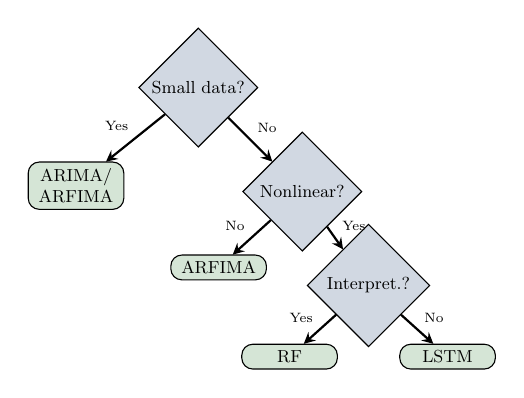
\begin{tikzpicture}[scale=0.7, transform shape,
        node distance=1cm,
        decision/.style={diamond, draw, fill=MainBlue!20, text width=1.8cm, align=center, inner sep=1pt, font=\small},
        block/.style={rectangle, draw, fill=Forest!20, text width=1.5cm, align=center, rounded corners, font=\small},
        arrow/.style={thick,->,>=stealth}
    ]
        \node[decision] (start) {Small data?};
        \node[block, below left=0.8cm and 0.8cm of start] (arima) {ARIMA/ ARFIMA};
        \node[decision, below right=0.8cm and 0.8cm of start] (nonlin) {Nonlinear?};
        \node[block, below left=0.6cm and 0.1cm of nonlin] (arfima) {ARFIMA};
        \node[decision, below right=0.6cm and 0.1cm of nonlin] (interp) {Interpret.?};
        \node[block, below left=0.5cm and 0cm of interp] (rf) {RF};
        \node[block, below right=0.5cm and 0cm of interp] (lstm) {LSTM};

        \draw[arrow] (start) -- node[above left, font=\scriptsize] {Yes} (arima);
        \draw[arrow] (start) -- node[above right, font=\scriptsize] {No} (nonlin);
        \draw[arrow] (nonlin) -- node[above left, font=\scriptsize] {No} (arfima);
        \draw[arrow] (nonlin) -- node[above right, font=\scriptsize] {Yes} (interp);
        \draw[arrow] (interp) -- node[above left, font=\scriptsize] {Yes} (rf);
        \draw[arrow] (interp) -- node[above right, font=\scriptsize] {No} (lstm);
    \end{tikzpicture}
    \end{center}
    \vspace{-0.1cm}
    {\small
    \begin{alertblock}{Trade-off}
        ML models offer better accuracy but higher computational cost. For small data or interpretability, ARIMA/ARFIMA remain excellent choices.
    \end{alertblock}
    }
    }
\end{frame}

\begin{frame}{Model Comparison: Accuracy vs Computational Cost}
    \vspace{-0.2cm}
    {\footnotesize
    \begin{block}{Interpretation}
            \begin{itemize}\setlength{\itemsep}{0pt}
                \item \textbf{Data}: EUR/RON daily exchange rate (Yahoo Finance, 2019--2025)
                \item \textbf{Trade-off}: ML models may achieve better accuracy, but computational cost increases significantly
                \item For small data or interpretability, ARIMA/ARFIMA remain excellent choices
            \end{itemize}
        \end{block}
    }
    \begin{center}
        \includegraphics[width=0.95\textwidth, height=0.50\textheight, keepaspectratio]{ch8_case_comparison.pdf}
    \end{center}
    \quantlet{TSA\_ch8\_model\_comparison}{https://github.com/QuantLet/TSA/tree/main/TSA_ch8/TSA_ch8_model_comparison}
\end{frame}

%=============================================================================
\section{Practical Applications}
%=============================================================================

\begin{frame}{Bitcoin: Price Evolution and Returns}
    \vspace{-0.2cm}
    {\footnotesize
    \begin{block}{Key Observations}
            \begin{itemize}\setlength{\itemsep}{0pt}
                \item Exponential price growth $\rightarrow$ strongly \textbf{leptokurtic} distribution
                \item Daily returns: mean $\approx 0.15\%$, volatility $\approx 3.5\%$
                \item Volatility clustering evident $\rightarrow$ crisis periods (2018, 2020, 2022)
                \item Kurtosis $\approx 10$--$15$ (well above the normal's 3)
            \end{itemize}
        \end{block}
    }
    \begin{center}
        \includegraphics[width=0.95\textwidth, height=0.46\textheight, keepaspectratio]{ch10_bitcoin_overview.pdf}
    \end{center}
    \quantlet{TSA\_ch10\_btc\_returns}{https://github.com/QuantLet/TSA/tree/main/TSA_ch10/TSA_ch10_btc_returns}
\end{frame}

\begin{frame}{Case Study: Bitcoin Price Forecasting}
    \begin{cminipage}{0.95\textwidth}
    \begin{block}{Why Bitcoin?}
        \begin{itemize}\setlength{\itemsep}{0pt}
            \item \textbf{Extreme} volatility and complex patterns
            \item Potential \textbf{long memory} in volatility
            \item \textbf{Nonlinear} relationships with exogenous variables
            \item Data available at \textbf{high frequency}
        \end{itemize}
    \end{block}
    \vspace{0.1cm}
    \begin{exampleblock}{Comparative Approach}
        \begin{enumerate}\setlength{\itemsep}{0pt}
            \item ARIMA on returns
            \item ARFIMA for long memory
            \item Random Forest with technical features
            \item LSTM on price sequences
        \end{enumerate}
    \end{exampleblock}
    \end{cminipage}
\end{frame}

\begin{frame}{Bitcoin: ACF and Evidence for Long Memory}
    \vspace{-0.2cm}
    {\footnotesize
    \begin{block}{ACF Analysis}
        \begin{itemize}\setlength{\itemsep}{0pt}
            \item ACF of returns: rapid decay $\rightarrow$ short memory in the mean
            \item ACF of squared returns: \textbf{slow, hyperbolic} decay
                \begin{itemize}\setlength{\itemsep}{0pt}
                    \item[$\blacktriangleright$] Indicates \textbf{long memory in volatility}
                    \item[$\blacktriangleright$] Hurst $H \approx 0.65$--$0.70$ ($d \approx 0.15$--$0.20$)
                \end{itemize}
            \item ARFIMA on volatility $>$ ARMA $\rightarrow$ captures shock persistence
        \end{itemize}
    \end{block}
    }
    \begin{center}
        \includegraphics[width=0.95\textwidth, height=0.43\textheight, keepaspectratio]{btc_acf_squared.pdf}
    \end{center}
    \quantlet{TSA\_ch10\_btc\_acf\_squared}{https://github.com/QuantLet/TSA/tree/main/TSA_ch10/TSA_ch10_btc_acf_squared}
\end{frame}

\begin{frame}{Bitcoin: GARCH and Risk Management}
    \vspace{-0.2cm}
    {\footnotesize
    {\small
        \begin{alertblock}{Conclusions -- Bitcoin Case Study}
            \begin{itemize}\setlength{\itemsep}{0pt}
                \item Differences between models are \textbf{small} for mean returns
                \item Major added value: \textbf{volatility modeling} (GARCH, EGARCH)
                \item ARFIMA captures volatility persistence (long memory)
                \item Random Forest: useful for \textbf{nonlinear features} (volume, sentiment)
                \item Optimal combination: ARFIMA-GARCH + exogenous features via RF
            \end{itemize}
        \end{alertblock}
        }
    }
    \begin{center}
        \includegraphics[width=0.95\textwidth, height=0.41\textheight, keepaspectratio]{ch10_bitcoin_garch.pdf}
    \end{center}
    \quantlet{TSA\_ch10\_garch\_forecast}{https://github.com/QuantLet/TSA/tree/main/TSA_ch10/TSA_ch10_garch_forecast}
\end{frame}

\begin{frame}{Bitcoin: ARFIMA Estimation and Model Comparison}
    \vspace{-0.2cm}
    \begin{columns}[T]
    \begin{column}{0.48\textwidth}
    {\footnotesize
    \begin{exampleblock}{BTC-USD Returns (2019--2024, test: 2024-02 -- 2024-12)}
        \begin{tabular}{lccc}
            \toprule
            \textbf{Model} & \textbf{RMSE} & \textbf{MAE} & \textbf{Interpr.?} \\
            \midrule
            ARIMA(1,0,1) & 2.81 & 2.05 & Yes \\
            ARFIMA(1,$d$,1) & 2.81 & 2.06 & Yes \\
            Random Forest & 2.84 & 2.07 & Partial \\
            LSTM & 2.94 & 2.13 & No \\
            \bottomrule
        \end{tabular}
    \end{exampleblock}
    \vspace{-0.15cm}
    {\scriptsize Hurst $\hat{d} = 0.13$; 70/15/15 temporal split}
    }
    \end{column}
    \begin{column}{0.50\textwidth}
        \includegraphics[width=\textwidth, height=0.50\textheight, keepaspectratio]{ch8_btc_model_comparison.pdf}
    \end{column}
    \end{columns}
    \quantlet{TSA\_ch8\_btc\_model\_comparison}{https://github.com/QuantLet/TSA/tree/main/TSA_ch8/TSA_ch8_btc_model_comparison}
\end{frame}

\begin{frame}{Energy: Demand Visualization and Multiple Seasonality}
    \vspace{-0.2cm}
    {\footnotesize
    \begin{block}{Identified Patterns}
            \begin{itemize}\setlength{\itemsep}{0pt}
                \item \textbf{Daily} (24h): peak morning (8--10) and evening (18--21), minimum at night
                \item \textbf{Weekly} (168h): reduced consumption on weekends ($\sim$15--20\% less)
                \item \textbf{Annual} (8766h): peak in summer (AC) and winter (heating)
                \item SARIMA cannot simultaneously model these 3 periods!
            \end{itemize}
        \end{block}
    }
    \begin{center}
        \includegraphics[width=0.95\textwidth, height=0.47\textheight, keepaspectratio]{ch9_electricity_demand.pdf}
    \end{center}
    \quantlet{TSA\_ch9\_electricity\_demand}{https://github.com/QuantLet/TSA/tree/main/TSA_ch9/TSA_ch9_electricity_demand}
\end{frame}

\begin{frame}{Case Study: Energy Consumption Forecasting}
    \begin{cminipage}{0.95\textwidth}
    \begin{block}{Characteristics}
        \begin{itemize}\setlength{\itemsep}{0pt}
            \item \textbf{Multiple seasonality}: daily, weekly, annual
            \item \textbf{Long-term trend} of growth
            \item \textbf{Exogenous variables}: temperature, holidays, price
            \item \textbf{Anomalies}: special events, outages
        \end{itemize}
    \end{block}
    \vspace{0.1cm}
    \begin{alertblock}{Challenges}
        \begin{itemize}\setlength{\itemsep}{0pt}
            \item Patterns at different temporal scales
            \item Complex interactions between variables
            \item Need for forecasts at different horizons
        \end{itemize}
    \end{alertblock}
    \end{cminipage}
\end{frame}

\begin{frame}{Energy: Why Prophet and TBATS?}
    \vspace{-0.2cm}
    {\footnotesize
    \begin{block}{Solution: Models with Multiple Seasonality}
        \begin{itemize}\setlength{\itemsep}{0pt}
            \item \textbf{TBATS}: periods $[24, 168, 8766]$ $\rightarrow$ Fourier for each season
                \begin{itemize}\setlength{\itemsep}{0pt}
                    \item[$\blacktriangleright$] Automatic, no manual tuning, good for production
                \end{itemize}
            \item \textbf{Prophet}: additive/multiplicative seasonality + regressors
                \begin{itemize}\setlength{\itemsep}{0pt}
                    \item[$\blacktriangleright$] Add temperature, holidays, special events
                \end{itemize}
            \item \textbf{Classical ARIMA}: can handle only 1 season $\rightarrow$ MAPE $\approx 8$--$10\%$
        \end{itemize}
    \end{block}
    }
    \begin{center}
        \includegraphics[width=0.95\textwidth, height=0.43\textheight, keepaspectratio]{ch9_multiple_seasonality.pdf}
    \end{center}
    \quantlet{TSA\_ch9\_multiple\_seasonality}{https://github.com/QuantLet/TSA/tree/main/TSA_ch9/TSA_ch9_multiple_seasonality}
\end{frame}

\begin{frame}{Energy: Prophet Decomposition and Results}
    \vspace{-0.2cm}
    {\footnotesize
    {\small
        \begin{exampleblock}{Comparison Results on Energy Data (MAPE)}
            \begin{center}
            \begin{tabular}{lcccc}
                \toprule
                \textbf{Model} & \textbf{MAPE} & \textbf{RMSE (MW)} & \textbf{95\% Coverage} \\
                \midrule
                SARIMA (1 season) & 8.5\% & 450 & 75\% \\
                TBATS & 4.2\% & 220 & 82\% \\
                Prophet & 4.8\% & 250 & 85\% \\
                Prophet + regressors & \textbf{3.9\%} & \textbf{200} & \textbf{88\%} \\
                \bottomrule
            \end{tabular}
            \end{center}
        \end{exampleblock}
        }
    }
    \begin{center}
        \includegraphics[width=0.95\textwidth, height=0.38\textheight, keepaspectratio]{ch9_prophet_vs_tbats.pdf}
    \end{center}
    \quantlet{TSA\_ch9\_prophet\_vs\_tbats}{https://github.com/QuantLet/TSA/tree/main/TSA_ch9/TSA_ch9_prophet_vs_tbats}
\end{frame}

\begin{frame}{Energy: Conclusions and Practical Recommendations}
    \begin{cminipage}{0.95\textwidth}
    \begin{block}{Lessons Learned}
        \begin{itemize}\setlength{\itemsep}{0pt}
            \item Models with \textbf{multiple seasonality} reduce MAPE by $\sim$50\% compared to SARIMA
            \item \textbf{Exogenous variables} (temperature) bring an additional 10--15\% gain
            \item Prophet excels at \textbf{interpretability}: trend + season + holiday decomposition
            \item TBATS: best \textbf{out-of-the-box} $\rightarrow$ no hyperparameter tuning needed
        \end{itemize}
    \end{block}
    \vspace{0.1cm}
    \begin{alertblock}{When to Choose Each Model?}
        \begin{itemize}\setlength{\itemsep}{0pt}
            \item \textbf{Prophet}: when you have external regressors + interpretation for management
            \item \textbf{TBATS}: automation, production, no human intervention
            \item \textbf{LSTM/RF}: if you have $>$100,000 observations and complex nonlinear patterns
        \end{itemize}
    \end{alertblock}
    {\footnotesize
    \begin{exampleblock}{}
        \textit{Full details on Prophet and TBATS $\rightarrow$ Chapter 9}
    \end{exampleblock}
    }
    \end{cminipage}
\end{frame}

%=============================================================================
% KEY FORMULAS SUMMARY
%=============================================================================
\begin{frame}{Key Formulas -- Summary}
    \begin{cminipage}{0.95\textwidth}
    \vspace{-0.3cm}
    {\scriptsize
            \begin{block}{ARFIMA(p,d,q)}
                $\phi(L)(1-L)^d Y_t = \theta(L)\varepsilon_t$ \quad $d \in (-0.5, 0.5)$: long memory
            \end{block}
            \vspace{-0.1cm}
            \begin{block}{Long Memory}
                \textbf{ACF}: $\rho_k \sim C \cdot k^{2d-1}$ \quad \textbf{Hurst}: $d = H - 0.5$ \quad $H > 0.5$: persistence
            \end{block}
            \vspace{-0.1cm}
            \begin{block}{Random Forest}
                $\hat{y} = \frac{1}{B}\sum_{b=1}^{B} T_b(x)$ \quad $B$ trees, random features
            \end{block}
            \vspace{-0.1cm}
            \begin{block}{LSTM Cell}
                $f_t = \sigma(W_f[h_{t-1}, x_t] + b_f)$ \quad $C_t = f_t \odot C_{t-1} + i_t \odot \tilde{C}_t$ \quad Forget, Input, Output gates
            \end{block}
            \vspace{-0.1cm}
            \begin{block}{Evaluation Metrics}
                RMSE $= \sqrt{\frac{1}{n}\sum(y_i - \hat{y}_i)^2}$ \quad MAPE $= \frac{100}{n}\sum\left|\frac{y_i - \hat{y}_i}{y_i}\right|$
            \end{block}
            \vspace{-0.1cm}
            \begin{block}{Time Series CV}
                Walk-forward validation --- Train $\rightarrow$ Test (temporal split)
            \end{block}
    }
    \end{cminipage}
\end{frame}

%=============================================================================
\section{Complete Case Study: EUR/RON Exchange Rate}
%=============================================================================

\begin{frame}{Case Study: EUR/RON Exchange Rate Forecasting}
    \begin{cminipage}{0.95\textwidth}
    \begin{block}{Why EUR/RON?}
        \begin{itemize}\setlength{\itemsep}{0pt}
            \item Relevance for the Romanian economy
            \item Potential \textbf{long memory} (shock persistence)
            \item Patterns influenced by \textbf{macroeconomic factors}
            \item Easily accessible data (BNR, Yahoo Finance)
        \end{itemize}
    \end{block}

    \vspace{0.2cm}

    \begin{exampleblock}{Objective}
        \begin{itemize}\setlength{\itemsep}{0pt}
            \item We compare ARIMA, ARFIMA, Random Forest, and LSTM on the same data to understand the strengths of each method
        \end{itemize}
    \end{exampleblock}
    \end{cminipage}
\end{frame}

\begin{frame}{EUR/RON Exchange Rate Visualization}
    \vspace{-0.2cm}
    {\footnotesize
    \begin{block}{Interpretation}
            \begin{itemize}\setlength{\itemsep}{0pt}
                \item \textbf{Data}: EUR/RON daily exchange rate (Yahoo Finance, 2019--2025)
                \item \textbf{Top}: EUR/RON rate --- depreciation trend and periods of high volatility
                \item \textbf{Bottom}: Daily returns --- volatility clustering (periods of high volatility are followed by similar periods)
            \end{itemize}
        \end{block}
    }
    \begin{center}
        \includegraphics[width=0.95\textwidth, height=0.50\textheight, keepaspectratio]{ch8_case_raw_data.pdf}
    \end{center}
    \quantlet{TSA\_ch8\_case\_raw\_data}{https://github.com/QuantLet/TSA/tree/main/TSA_ch8/TSA_ch8_case_raw_data}
\end{frame}

\begin{frame}{ACF Analysis: Returns vs Squared Returns}
    \vspace{-0.2cm}
    {\footnotesize
    \begin{block}{Interpretation}
            \begin{itemize}\setlength{\itemsep}{0pt}
                \item \textbf{Data}: EUR/RON daily returns and squared returns (Yahoo Finance, 2019--2025)
                \item \textbf{Left}: ACF of returns --- rapid decay, no significant autocorrelation after lag 1
                \item \textbf{Right}: ACF of squared returns --- slow decay indicates \textbf{volatility clustering} (ARCH effects)
            \end{itemize}
        \end{block}
    }
    \begin{center}
        \includegraphics[width=0.95\textwidth, height=0.50\textheight, keepaspectratio]{ch8_case_acf_analysis.pdf}
    \end{center}
    \quantlet{TSA\_ch8\_case\_acf\_analysis}{https://github.com/QuantLet/TSA/tree/main/TSA_ch8/TSA_ch8_case_acf_analysis}
\end{frame}

\begin{frame}{Long Memory Test Results -- EUR/RON}
    \begin{cminipage}{0.95\textwidth}
    \begin{block}{Typical Output}
        {\footnotesize
        \begin{itemize}\setlength{\itemsep}{0pt}
            \item \texttt{Phillips-Perron p-value: 0.0001} (returns are stationary)
            \item \texttt{Hurst Exponent (H): 0.47}
            \item \texttt{Estimated parameter d: -0.03}
            \item \texttt{Slightly ANTI-PERSISTENT series (mean-reverting)}
        \end{itemize}
        }
    \end{block}

    \vspace{0.2cm}

    \begin{alertblock}{Interpretation}
        \begin{itemize}\setlength{\itemsep}{0pt}
            \item EUR/RON returns are \textbf{stationary} (p-value $< 0.05$)
            \item $H \approx 0.47 < 0.5$: slight mean-reversion tendency
            \item $d \approx 0$: \textbf{short memory} -- ARMA may be sufficient
            \item However, \textbf{volatility} may have long memory!
        \end{itemize}
    \end{alertblock}
    \end{cminipage}
\end{frame}

\begin{frame}{Random Forest: Feature Importance}
    \vspace{-0.2cm}
    {\footnotesize
    \begin{block}{Interpretation}
            \begin{itemize}\setlength{\itemsep}{0pt}
                \item \textbf{Data}: EUR/RON exchange rate (Yahoo Finance, 2019--2025) --- RF with 10 engineered features
                \item Recent lags (lag\_1, lag\_2) and rolling volatility are the most important features
                \item Calendar features have minor impact for daily return prediction
            \end{itemize}
        \end{block}
    }
    \begin{center}
        \includegraphics[width=0.95\textwidth, height=0.50\textheight, keepaspectratio]{ch8_case_feature_importance.pdf}
    \end{center}
    \quantlet{TSA\_ch8\_case\_feature\_importance}{https://github.com/QuantLet/TSA/tree/main/TSA_ch8/TSA_ch8_case_feature_importance}
\end{frame}

\begin{frame}{LSTM: Learning Curve}
    \vspace{-0.2cm}
    {\footnotesize
    \begin{block}{Interpretation}
            \begin{itemize}\setlength{\itemsep}{0pt}
                \item \textbf{Data}: EUR/RON exchange rate (Yahoo Finance, 2019--2025) --- Neural Network (100 epochs, MSE loss)
                \item \textbf{Training Loss}: Decreases rapidly in early epochs, then stabilizes
                \item \textbf{Validation Loss}: Tracks training loss --- no severe overfitting
            \end{itemize}
        \end{block}
    }
    \begin{center}
        \includegraphics[width=0.95\textwidth, height=0.47\textheight, keepaspectratio]{ch8_case_lstm_training.pdf}
    \end{center}
    \quantlet{TSA\_ch8\_case\_lstm\_training}{https://github.com/QuantLet/TSA/tree/main/TSA_ch8/TSA_ch8_case_lstm_training}
\end{frame}

%=============================================================================
\section{Final Comparison: All Methods}
%=============================================================================

\begin{frame}{Visualization: Predictions vs Actual Values}
    \vspace{-0.2cm}
    {\footnotesize
    \begin{block}{Interpretation}
            \begin{itemize}\setlength{\itemsep}{0pt}
                \item \textbf{Data}: EUR/RON test period --- ARIMA, Random Forest, MLP/LSTM predictions vs actual values
                \item All models capture the general pattern, but none perfectly predicts volatility spikes
                \item This reflects \textbf{market efficiency} and \textbf{prediction limits} for financial series
            \end{itemize}
        \end{block}
    }
    \begin{center}
        \includegraphics[width=0.95\textwidth, height=0.50\textheight, keepaspectratio]{ch8_case_predictions.pdf}
    \end{center}
    \quantlet{TSA\_ch8\_case\_predictions}{https://github.com/QuantLet/TSA/tree/main/TSA_ch8/TSA_ch8_case_predictions}
\end{frame}

\begin{frame}{Comparison: Results on EUR/RON}
    \begin{cminipage}{0.95\textwidth}
    \begin{center}
    \begin{tabular}{l|c|c|c|c}
        \toprule
        \textbf{Model} & \textbf{RMSE} & \textbf{MAE} & \textbf{Time (s)} & \textbf{Interpretable?} \\
        \midrule
        ARIMA(1,1,1) & 0.0069 & 0.0062 & 0.08 & Yes \\
        Random Forest & 0.0057 & 0.0050 & 0.51 & Yes (features) \\
        MLP/LSTM & 0.0071 & 0.0059 & 0.47 & No \\
        \bottomrule
    \end{tabular}
    \end{center}

    \vspace{0.1cm}

    \begin{alertblock}{Conclusions}
        \begin{itemize}\setlength{\itemsep}{0pt}
            \item For EUR/RON, the differences are \textbf{small} -- the market is efficient
            \item Random Forest offers the best \textbf{accuracy/interpretability} trade-off
            \item LSTM has high computational cost for marginal gain
            \item ARIMA remains a solid choice for \textbf{baseline}
        \end{itemize}
    \end{alertblock}
    \end{cminipage}
\end{frame}

\begin{frame}{Model Comparison: Performance Metrics}
    \vspace{-0.2cm}
    {\footnotesize
    \begin{block}{Interpretation}
            \begin{itemize}\setlength{\itemsep}{0pt}
                \item \textbf{Data}: EUR/RON exchange rate (Yahoo Finance, 2019--2025) --- ARIMA vs RF vs MLP/LSTM
                \item \textbf{Left}: Error metrics (lower = better) --- RF achieves the lowest RMSE and MAE
                \item \textbf{Right}: Training time (log scale) --- ML models require more computational resources
            \end{itemize}
        \end{block}
    }
    \begin{center}
        \includegraphics[width=0.95\textwidth, height=0.50\textheight, keepaspectratio]{ch8_case_comparison.pdf}
    \end{center}
    \quantlet{TSA\_ch8\_case\_comparison}{https://github.com/QuantLet/TSA/tree/main/TSA_ch8/TSA_ch8_case_comparison}
\end{frame}

%=============================================================================
% CASE STUDY 2: Energy Consumption
%=============================================================================
\section{Case Study 2: Energy Consumption}

\begin{frame}{Case Study: Data Overview}
    \vspace{-0.2cm}
    {\scriptsize
    \begin{block}{Interpretation}
        \begin{itemize}\setlength{\itemsep}{0pt}
            \item \textbf{Train}: 1513 obs (70\%) \quad \textbf{Validation}: 324 obs (15\%) \quad \textbf{Test}: 325 obs (15\%)
        \end{itemize}
    \end{block}
    }
    \begin{center}
        \includegraphics[width=0.95\textwidth, height=0.50\textheight, keepaspectratio]{ch8_data_split.pdf}
    \end{center}
    \quantlet{TSA\_ch8\_data\_split}{https://github.com/QuantLet/TSA/tree/main/TSA_ch8/TSA_ch8_data_split}
\end{frame}

\begin{frame}{Case Study: Model Predictions}
    \begin{cminipage}{0.95\textwidth}
    \vspace{-0.2cm}
    {\footnotesize
    \begin{center}
    \begin{tabular}{l|c|c|l}
        \textbf{Rank} & \textbf{Model} & \textbf{MAPE} & \textbf{Interpretation} \\
        \hline
        1 & \textcolor{Forest}{\textbf{Random Forest}} & \textcolor{Forest}{\textbf{2.2\%}} & Best: captures nonlinear patterns \\
        2 & \textcolor{IDAred}{\textbf{LSTM}} & \textcolor{IDAred}{\textbf{3.3\%}} & Good, needs more data \\
        3 & \textcolor{AccentBlue}{\textbf{Baseline}} & \textcolor{AccentBlue}{\textbf{3.9\%}} & Simple but competitive \\
        4 & \textcolor{Orange}{\textbf{ARFIMA}} & \textcolor{Orange}{\textbf{12.3\%}} & Long memory not sufficient \\
        5 & \textcolor{Purple}{\textbf{SARIMA}} & \textcolor{Purple}{\textbf{14.6\%}} & Struggles with patterns \\
    \end{tabular}
    \end{center}
    }
    \begin{center}
        \includegraphics[width=0.95\textwidth, height=0.50\textheight, keepaspectratio]{ch8_model_predictions.pdf}
    \end{center}

    \quantlet{TSA\_ch8\_model\_predictions}{https://github.com/QuantLet/TSA/tree/main/TSA_ch8/TSA_ch8_model_predictions}
    \end{cminipage}
\end{frame}

\begin{frame}{Case Study: Best Model Performance}
    \begin{center}
        \includegraphics[width=0.95\textwidth, height=0.78\textheight, keepaspectratio]{ch8_best_model_prediction.pdf}
    \end{center}
    \quantlet{TSA\_ch8\_best\_model}{https://github.com/QuantLet/TSA/tree/main/TSA_ch8/TSA_ch8_best_model}
\end{frame}

\begin{frame}{When to Choose Each Model?}
    \begin{cminipage}{0.95\textwidth}
    \vspace{-0.2cm}
    {\small
            \begin{block}{ARIMA/ARFIMA}
                \begin{itemize}\setlength{\itemsep}{0pt}
                    \item Few data ($< 500$ obs.), interpretation important, suspected long memory, quick baseline
                \end{itemize}
            \end{block}

            \begin{block}{Random Forest}
                \begin{itemize}\setlength{\itemsep}{0pt}
                    \item Many exogenous variables, nonlinear relationships, feature importance, moderate data
                \end{itemize}
            \end{block}

            \begin{block}{LSTM/Deep Learning}
                \begin{itemize}\setlength{\itemsep}{0pt}
                    \item Very large data ($> 10,000$), complex sequences, computational resources, hidden patterns
                \end{itemize}
            \end{block}

            \begin{alertblock}{Golden Rule}
                \begin{itemize}\setlength{\itemsep}{0pt}
                    \item Start simple (ARIMA), add complexity only if performance increases significantly!
                \end{itemize}
            \end{alertblock}
    }
    \end{cminipage}
\end{frame}

%=============================================================================
\section{Additional Examples with Real Data}
%=============================================================================

\begin{frame}{Example 2: BET Index (Bucharest Stock Exchange)}
    \begin{cminipage}{0.95\textwidth}
    \begin{block}{Characteristics}
        \begin{itemize}\setlength{\itemsep}{0pt}
            \item Strong \textbf{volatility clustering}
            \item Influenced by international markets
            \item Lower liquidity than developed markets
            \item Potential for long memory in volatility
        \end{itemize}
    \end{block}

    \vspace{0.2cm}

    \begin{exampleblock}{Typical Results (RMSE on returns)}
        \begin{itemize}\setlength{\itemsep}{0pt}
            \item GARCH(1,1): 1.45 -- best for volatility
            \item ARFIMA for volatility: 1.52
            \item Random Forest: 1.48
            \item LSTM: 1.51
        \end{itemize}
    \end{exampleblock}
    \end{cminipage}
\end{frame}

\begin{frame}{Example 3: Romania Inflation Rate}
    \begin{cminipage}{0.95\textwidth}
    \begin{block}{Characteristics}
        \begin{itemize}\setlength{\itemsep}{0pt}
            \item \textbf{Monthly} series (low frequency)
            \item \textbf{High persistence} -- shocks last long
            \item Influenced by monetary policy
            \item Strong potential for \textbf{long memory}
        \end{itemize}
    \end{block}

    \vspace{0.1cm}

    \begin{alertblock}{Typical Results}
        \begin{itemize}\setlength{\itemsep}{0pt}
            \item ARFIMA with $d \approx 0.35$ -- captures persistence
            \item ARIMA underestimates shock persistence
            \item ML does not work well (few data, ~300 obs.)
        \end{itemize}
    \end{alertblock}

    \vspace{0.2cm}

    {\footnotesize
    \begin{exampleblock}{}
        \begin{itemize}\setlength{\itemsep}{0pt}
            \item \textbf{Lesson}: For monthly series with few data, classical models (ARFIMA) are superior!
        \end{itemize}
    \end{exampleblock}
    }
    \end{cminipage}
\end{frame}

\begin{frame}{Practical Summary: Model Selection}
    \begin{cminipage}{0.95\textwidth}
    \begin{center}
    \begin{tabular}{l|c|c|c|c}
        \toprule
        \textbf{Criterion} & \textbf{ARIMA} & \textbf{ARFIMA} & \textbf{RF} & \textbf{LSTM} \\
        \midrule
        Data needed & Few & Few & Medium & Many \\
        Long memory & No & \textbf{Yes} & Partial & Partial \\
        Nonlinearity & No & No & \textbf{Yes} & \textbf{Yes} \\
        Interpretability & \textbf{Yes} & \textbf{Yes} & Partial & No \\
        Computation time & Fast & Fast & Medium & Slow \\
        Exog. variables & Limited & Limited & \textbf{Yes} & \textbf{Yes} \\
        \bottomrule
    \end{tabular}
    \end{center}

    \vspace{0.1cm}

    \begin{block}{Recommended Workflow}
        \begin{enumerate}\setlength{\itemsep}{0pt}
            \item Start with \textbf{ARIMA} as baseline
            \item Test for \textbf{long memory} $\rightarrow$ ARFIMA if $d$ is significant
            \item Add \textbf{features} $\rightarrow$ Random Forest
            \item Only with lots of data and resources $\rightarrow$ LSTM
        \end{enumerate}
    \end{block}
    \end{cminipage}
\end{frame}

%=============================================================================
\section{AI Use Case}
%=============================================================================

\begin{frame}{AI Exercise: Critical Thinking}
    \begin{cminipage}{0.95\textwidth}
    \vspace{-3mm}
    \begin{block}{\footnotesize Prompt to test in ChatGPT / Claude / Copilot}
        {\footnotesize
        ``Using yfinance, download daily Bitcoin prices (BTC-USD) from 2019-01-01 to 2024-12-31 (approx.\ 2{,}200 observations). Compute daily percentage returns. Compare ARIMA, Random Forest, and LSTM for 7-day-ahead forecasting using a 70/15/15 temporal split. Which model is best? Give me complete Python code with comparison charts.''
        }
    \end{block}
    \vspace{-2mm}
    {\footnotesize
    \textbf{Exercise}:
    \begin{enumerate}\setlength{\itemsep}{0pt}
        \item Run the prompt in an LLM of your choice and critically analyze the response.
        \item How are features engineered for Random Forest? Lags, calendar variables, Fourier terms?
        \item Is the LSTM properly structured? Input shape, scaling, train/test split without leakage?
        \item Does it use walk-forward validation or just a single train/test split?
        \item Does it mention interpretability and computational cost trade-offs?
    \end{enumerate}
    }
    \vspace{-2mm}
    \begin{alertblock}{}
        {\footnotesize \textbf{Warning}: AI-generated code may run without errors and look professional. \textit{That does not mean it is correct.}}
    \end{alertblock}
    \end{cminipage}
\end{frame}

%=============================================================================
\section{Summary}
%=============================================================================

\begin{frame}{Summary}
    \begin{cminipage}{0.95\textwidth}
    \begin{block}{What We Learned}
        \begin{itemize}\setlength{\itemsep}{0pt}
            \item \textbf{ARFIMA}: Extends ARIMA for long memory (fractional $d$)
            \item \textbf{Random Forest}: Ensemble of trees, nonlinear relationships, interpretable
            \item \textbf{LSTM}: Deep learning for sequences, complex dependencies
            \item \textbf{Trade-offs}: Complexity vs interpretability vs data requirements
        \end{itemize}
    \end{block}

    \vspace{0.2cm}

    \begin{alertblock}{Practical Recommendations}
        \begin{itemize}\setlength{\itemsep}{0pt}
            \item Start with \textbf{simple} models (ARIMA) as baseline
            \item Use \textbf{Time Series CV} for proper evaluation
            \item ML requires careful \textbf{feature engineering}
            \item LSTM: only with \textbf{lots of data} and computational resources
        \end{itemize}
    \end{alertblock}
    \end{cminipage}
\end{frame}

%=============================================================================
\section{Quiz}
%=============================================================================

\begin{frame}{Question 1}
    \begin{cminipage}{0.95\textwidth}
    \begin{alertblock}{Question}
        \begin{itemize}\setlength{\itemsep}{0pt}
            \item What does $d = 0.3$ mean in an ARFIMA model?
        \end{itemize}
    \end{alertblock}

    \vspace{0.3cm}

    \begin{block}{Answer Choices}

        \textcolor{MainBlue}{\textbf{(A)}} The series needs 0.3 differences to become stationary\\[3pt]

        \textcolor{MainBlue}{\textbf{(B)}} Long memory: stationary but ACF decays hyperbolically (slowly)\\[3pt]

        \textcolor{MainBlue}{\textbf{(C)}} The series is non-stationary with a unit root\\[3pt]

        \textcolor{MainBlue}{\textbf{(D)}} Short memory: ACF decays exponentially (fast)

    \end{block}
    \end{cminipage}
\end{frame}

\begin{frame}{Question 1: Answer}
    \begin{cminipage}{0.95\textwidth}
    \vspace{-0.2cm}
    \begin{center}
        \includegraphics[width=0.98\textwidth, height=0.58\textheight, keepaspectratio]{ch8_quiz1_long_memory.pdf}
    \end{center}
    \vspace{-3mm}
    {\small
    \begin{exampleblock}{Answer: (B)}
    \begin{itemize}\setlength{\itemsep}{0pt}
        \item For $0 < d < 0.5$: stationary but ACF $\sim k^{2d-1}$ decays much slower than exponential. This ``long memory'' means distant observations still matter.
    \end{itemize}
    \end{exampleblock}
    }
    \hfill\quantlet{TSA\_ch8\_quiz1\_long\_memory}{https://github.com/QuantLet/TSA/tree/main/TSA_ch8/TSA_ch8_quiz1_long_memory}
    \end{cminipage}
\end{frame}

\begin{frame}{Question 2}
    \begin{cminipage}{0.95\textwidth}
    \begin{alertblock}{Question}
        \begin{itemize}\setlength{\itemsep}{0pt}
            \item Why should you use Time Series Cross-Validation instead of standard k-fold?
        \end{itemize}
    \end{alertblock}

    \vspace{0.3cm}

    \begin{block}{Answer Choices}

        \textcolor{MainBlue}{\textbf{(A)}} k-fold is computationally more expensive\\[3pt]

        \textcolor{MainBlue}{\textbf{(B)}} Time Series CV uses more training data\\[3pt]

        \textcolor{MainBlue}{\textbf{(C)}} k-fold violates temporal order, causing data leakage\\[3pt]

        \textcolor{MainBlue}{\textbf{(D)}} There is no difference; both methods are equivalent

    \end{block}
    \end{cminipage}
\end{frame}

\begin{frame}{Question 2: Answer}
    \begin{cminipage}{0.95\textwidth}
    \vspace{-0.2cm}
    \begin{center}
        \includegraphics[width=0.98\textwidth, height=0.58\textheight, keepaspectratio]{ch8_quiz2_timeseries_cv.pdf}
    \end{center}
    \vspace{-3mm}
    {\small
    \begin{exampleblock}{Answer: (C)}
    \begin{itemize}\setlength{\itemsep}{0pt}
        \item Standard k-fold randomly shuffles data, using future observations to predict past ones. Time Series CV always trains on past and tests on future, respecting causality.
    \end{itemize}
    \end{exampleblock}
    }
    \hfill\quantlet{TSA\_ch8\_quiz2\_timeseries\_cv}{https://github.com/QuantLet/TSA/tree/main/TSA_ch8/TSA_ch8_quiz2_timeseries_cv}
    \end{cminipage}
\end{frame}

\begin{frame}{Question 3}
    \begin{cminipage}{0.95\textwidth}
    \begin{alertblock}{Question}
        \begin{itemize}\setlength{\itemsep}{0pt}
            \item What is the main advantage of LSTM over simple RNNs?
        \end{itemize}
    \end{alertblock}

    \vspace{0.3cm}

    \begin{block}{Answer Choices}

        \textcolor{MainBlue}{\textbf{(A)}} LSTM uses fewer parameters\\[3pt]

        \textcolor{MainBlue}{\textbf{(B)}} LSTM solves the vanishing gradient problem via gating mechanisms\\[3pt]

        \textcolor{MainBlue}{\textbf{(C)}} LSTM is faster to train\\[3pt]

        \textcolor{MainBlue}{\textbf{(D)}} LSTM does not require sequential data

    \end{block}
    \end{cminipage}
\end{frame}

\begin{frame}{Question 3: Answer}
    \begin{cminipage}{0.95\textwidth}
    \vspace{-0.2cm}
    \begin{center}
        \includegraphics[width=0.98\textwidth, height=0.58\textheight, keepaspectratio]{ch8_quiz3_lstm_gates.pdf}
    \end{center}
    \vspace{-3mm}
    {\small
    \begin{exampleblock}{Answer: (B)}
    \begin{itemize}\setlength{\itemsep}{0pt}
        \item LSTM's forget, input, and output gates control information flow, preserving gradients across long sequences. Simple RNNs lose gradient signal after $\sim$10--20 steps.
    \end{itemize}
    \end{exampleblock}
    }
    \hfill\quantlet{TSA\_ch8\_quiz3\_lstm\_gates}{https://github.com/QuantLet/TSA/tree/main/TSA_ch8/TSA_ch8_quiz3_lstm_gates}
    \end{cminipage}
\end{frame}

\begin{frame}{Question 4}
    \begin{cminipage}{0.95\textwidth}
    \begin{alertblock}{Question}
        \begin{itemize}\setlength{\itemsep}{0pt}
            \item You have a small dataset (100 observations) with linear relationships. Which model is most appropriate?
        \end{itemize}
    \end{alertblock}

    \vspace{0.3cm}

    \begin{block}{Answer Choices}

        \textcolor{MainBlue}{\textbf{(A)}} LSTM --- deep learning captures all patterns\\[3pt]

        \textcolor{MainBlue}{\textbf{(B)}} Random Forest --- handles any relationship\\[3pt]

        \textcolor{MainBlue}{\textbf{(C)}} ARIMA/ARFIMA --- parsimonious and effective with small data\\[3pt]

        \textcolor{MainBlue}{\textbf{(D)}} Ensemble of all models for best accuracy

    \end{block}
    \end{cminipage}
\end{frame}

\begin{frame}{Question 4: Answer}
    \begin{cminipage}{0.95\textwidth}
    \vspace{-0.2cm}
    \begin{center}
        \includegraphics[width=0.98\textwidth, height=0.58\textheight, keepaspectratio]{ch8_quiz4_model_complexity.pdf}
    \end{center}
    \vspace{-3mm}
    {\small
    \begin{exampleblock}{Answer: (C)}
    \begin{itemize}\setlength{\itemsep}{0pt}
        \item ML models (RF, LSTM) need large datasets to generalize. With 100 observations and linear dynamics, ARIMA's few parameters avoid overfitting and often outperform complex models.
    \end{itemize}
    \end{exampleblock}
    }
    \hfill\quantlet{TSA\_ch8\_quiz4\_model\_complexity}{https://github.com/QuantLet/TSA/tree/main/TSA_ch8/TSA_ch8_quiz4_model_complexity}
    \end{cminipage}
\end{frame}

\begin{frame}{Question 5}
    \begin{cminipage}{0.95\textwidth}
    \begin{alertblock}{Question}
        \begin{itemize}\setlength{\itemsep}{0pt}
            \item What is ``data leakage'' in the context of ML for time series?
        \end{itemize}
    \end{alertblock}

    \vspace{0.3cm}

    \begin{block}{Answer Choices}

        \textcolor{MainBlue}{\textbf{(A)}} Missing values in the dataset\\[3pt]

        \textcolor{MainBlue}{\textbf{(B)}} Using future information in features or during training\\[3pt]

        \textcolor{MainBlue}{\textbf{(C)}} Having too many features relative to observations\\[3pt]

        \textcolor{MainBlue}{\textbf{(D)}} The model memorizing the training data

    \end{block}
    \end{cminipage}
\end{frame}

\begin{frame}{Question 5: Answer}
    \begin{cminipage}{0.95\textwidth}
    \vspace{-0.2cm}
    \begin{center}
        \includegraphics[width=0.98\textwidth, height=0.58\textheight, keepaspectratio]{ch8_quiz5_data_leakage.pdf}
    \end{center}
    \vspace{-3mm}
    {\small
    \begin{exampleblock}{Answer: (B)}
    \begin{itemize}\setlength{\itemsep}{0pt}
        \item Examples: centered moving averages (use future values), standard k-fold (mixes temporal order), computing statistics over the full dataset before splitting.
    \end{itemize}
    \end{exampleblock}
    }
    \hfill\quantlet{TSA\_ch8\_quiz5\_data\_leakage}{https://github.com/QuantLet/TSA/tree/main/TSA_ch8/TSA_ch8_quiz5_data_leakage}
    \end{cminipage}
\end{frame}

\begin{frame}{What Comes Next?}
    \begin{cminipage}{0.95\textwidth}
    \begin{block}{Extensions and Advanced Topics}
        \begin{itemize}\setlength{\itemsep}{0pt}
            \item \textbf{Transformer} for time series (Temporal Fusion Transformer)
            \item \textbf{Prophet} (Facebook/Meta) for seasonality
            \item \textbf{Neural Prophet}: Prophet + neural networks
            \item \textbf{Ensemble methods}: Combining multiple models
            \item \textbf{Anomaly detection} with ML
        \end{itemize}
    \end{block}

    \vspace{0.1cm}

    \begin{center}
        \Large\textcolor{MainBlue}{Questions?}
    \end{center}
    \end{cminipage}
\end{frame}


%=============================================================================
% BIBLIOGRAPHY
%=============================================================================
\begin{frame}{Bibliography I}
    \begin{block}{Long Memory and ARFIMA}
        {\small
        \begin{itemize}\setlength{\itemsep}{0pt}
            \item Granger, C.W.J., \& Joyeux, R. (1980). An Introduction to Long-Memory Time Series Models and Fractional Differencing, \textit{Journal of Time Series Analysis}, 1(1), 15--29.
            \item Baillie, R.T. (1996). Long Memory Processes and Fractional Integration in Econometrics, \textit{Journal of Econometrics}, 73(1), 5--59.
            \item Beran, J. (1994). \textit{Statistics for Long-Memory Processes}, Chapman \& Hall.
        \end{itemize}
        }
    \end{block}

    \begin{exampleblock}{Neural Networks and Deep Learning for Time Series}
        {\small
        \begin{itemize}\setlength{\itemsep}{0pt}
            \item Hochreiter, S., \& Schmidhuber, J. (1997). Long Short-Term Memory, \textit{Neural Computation}, 9(8), 1735--1780.
            \item Bai, J., \& Perron, P. (2003). Computation and Analysis of Multiple Structural Change Models, \textit{Journal of Applied Econometrics}, 18(1), 1--22.
        \end{itemize}
        }
    \end{exampleblock}
\end{frame}

\begin{frame}{Bibliography II}
    \begin{block}{Threshold and Regime-Switching Models}
        {\small
        \begin{itemize}\setlength{\itemsep}{0pt}
            \item Hansen, B.E. (2011). Threshold Autoregression in Economics, \textit{Statistics and Its Interface}, 4(2), 123--127.
            \item Hamilton, J.D. (1989). A New Approach to the Economic Analysis of Nonstationary Time Series and the Business Cycle, \textit{Econometrica}, 57(2), 357--384.
            \item Petropoulos, F., et al. (2022). Forecasting: Theory and Practice, \textit{International Journal of Forecasting}, 38(3), 845--1054.
        \end{itemize}
        }
    \end{block}

    \begin{exampleblock}{Online Resources and Code}
        {\small
        \begin{itemize}\setlength{\itemsep}{0pt}
            \item \textbf{Quantlet}: \url{https://quantlet.com} $\succ$ Code repository for statistics
            \item \textbf{Quantinar}: \url{https://quantinar.com} $\succ$ Learning platform for quantitative methods
            \item \textbf{GitHub TSA}: \url{https://github.com/QuantLet/TSA/tree/main/TSA_ch8} $\succ$ Python code for this chapter
        \end{itemize}
        }
    \end{exampleblock}
\end{frame}

\begin{frame}{}
    \centering
    \Huge\textcolor{MainBlue}{Thank You!}

    \vspace{1cm}

    \Large Questions?

    \vspace{0.8cm}

    \normalsize

    Course materials available at: \url{https://danpele.github.io/Time-Series-Analysis/}

    \vspace{0.2cm}

    \href{https://quantlet.com}{\raisebox{-0.15em}{\includegraphics[height=0.8em]{ql_logo.png}} Quantlet} \hspace{0.5cm}
    \href{https://quantinar.com}{\raisebox{-0.15em}{\includegraphics[height=0.8em]{qr_logo.png}} Quantinar}
\end{frame}

\end{document}
